\documentclass{programmierpraktikum}
\vorlesung{Programmierpraktikum}
\semester{Sommersemester 2013}
\betreuer{Wilfried Linder}
\subtitle{Dungeon Crawler}

\begin{document}
%
\maketitle
In diesem Jahr soll ein \textbf{Dungeon Crawler} programmiert werden. Aussehen, Thema und auch
verschiedene Komponenten des Gameplays sind dabei frei wählbar. Zum ersten Meilenstein gibt es
jedoch noch relativ klare Vorgaben.
%
\section{Spielprinzip nach Wikipedia}
Wie in der Namensgebung schon angedeutet, entfalten Dungeons üblicherweise eine gruselige
Atmosphäre, oft sind sie als Katakomben oder ausgebaute Höhlensysteme gestaltet, manchmal auch
als unterirdische Labyrinthe, die absichtlich als Versteck für Schätze und als Aufenthaltsort
für Monster angelegt wurden. Manchmal wird der Begriff Dungeon abweichend von der eigentlichen
Wortbedeutung auch auf Gebäude und andere oberirdische Schauplätze ausgedehnt, wenn sie spieltechnisch
demselben Zweck dienen.
%
\section{Mindestanforderungen \& erster Meilenstein}
%
\begin{figure}[h!]
  \begin{center}
    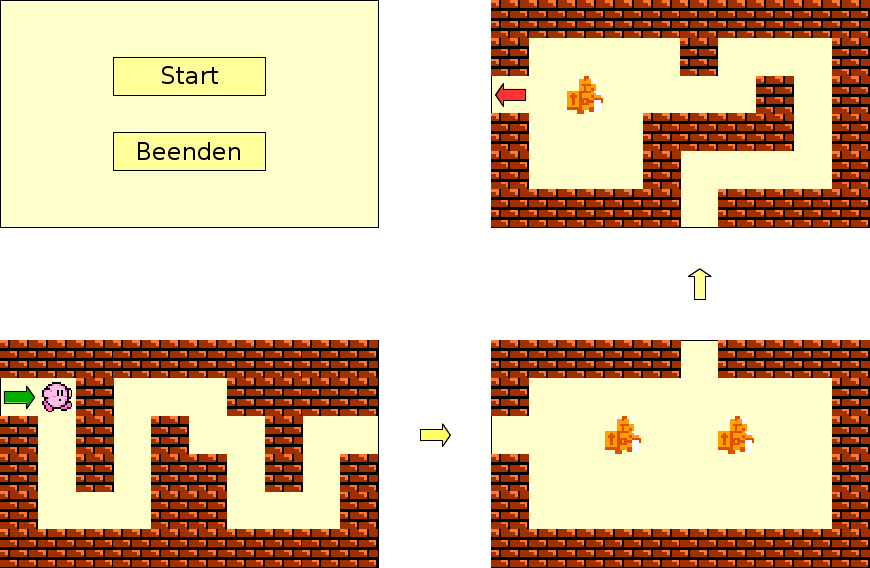
\includegraphics[width=.75\textwidth]{skizze}
    \caption{Erster Meilenstein\label{fig:skizze}}
  \end{center}
\end{figure}
Für den ersten Meilenstein müssen bereits bestimmte Mindestanforderungen erfüllt werden:
\begin{enumerate}
  \item Darstellung eines Spielfelds in 2D.
  \item Steuerung einer Figur durch das Spielfeld.
  \item 3 feste Räume mit festen Wänden (Hindernissen) und Ein-/Ausgängen
  \item Ziel im letzten Raum
  \item Feste Gegner/Fallen, die bei Berührung zur Niederlage führen
  \item Automatisches Neustarten eines Spiels nach Sieg oder Niederlage, Menüführung.
\end{enumerate}
Eine grobe Skizzierung finden Sie in Abb.~\ref{fig:skizze}. Sie brauchen (sollen) sich nicht an der
grafischen Gestaltung orientieren. Diese steht ihnen vollkommen frei. Das gilt auch für die
Anordung der Wände, Ein- und Ausgänge und Gegner.

Stichtag für den ersten Meilenstein ist der \textbf{Übungstermin in der Woche vom 20. -- 24. Mai 2013}
%
\section{Hinweise}
\begin{itemize}
  \item Für die schnelle grafische Arbeit ist die Verwendung von
    StdDraw.java\footnote{\url{http://introcs.cs.princeton.edu/java/stdlib/StdDraw.java.html}} erlaubt
    bzw. empfohlen.
  \item Als zentrales Repository für die Versionierung steht uns Github zur Verfügung.
  \item Die Adresse für das Gruppen-Repository lautet:\\
    \textbf{http://github.com/propra13-orga/gruppe<gruppen-nr>}
  \item Die URL für den Remote lautet:\\
    \textbf{git@github.com:propra13-orga/gruppe<gruppen-nr>}
  \item Die Gruppen-Nummer wird in den Übungsgruppen verteilt.
\end{itemize}
%
\section{Zusatzanforderungen}
Zusätzlich zu diesen Anforderungen wird es im Laufe des Praktikums einen Katalog weiterer
Anforderungen geben, von denen einzelne ausgewählt und implementiert werden sollen. Dabei werden
auch frei gewählte Erweiterungen erlaubt sein, wobei die Wertung dann in Absprache mit dem
Übungsgruppenleiter erfolgt. Es lohnt sich also, bis zum ersten Meilenstein bereits mehr als die
Mindestanforderungen zu erfüllen.

\textbf{Beispiele}
\begin{itemize}
  \item Steuerung einer weiteren Spielfigur (Tastatur, Netzwerk, Computergegner)
  \item Implementierung verschiedener Gegenstände (Waffen, Rüstungen)
  \item Implementierung von Lebenspunkten für die Spielfigur
  \item Einlesen der Level aus Dateien
\end{itemize}
\emph{Diese Anforderungen sind Zusatzanforderungen und müssen zum ersten Meilenstein nicht erfüllt sein!}
%
\section{Formales}
Abgesehen von den inhaltlichen Anforderungen gibt es noch einige formale Anforderungen an das Projekt:
\begin{itemize}
  \item Die Implementierung erfolgt in Java, wenn nicht anders abgesprochen. Weitere
    Programmiersprachen sind erlaubt. Da aber nicht jeder Tutor jede Sprache beherrscht und im
    Zweifelsfall Support leisten kann, muss eine von Java abweichende Wahl der Programmiersprache
    mit uns abgesprochen werden.
  \item Die Verwendung von Bibliotheken, die nicht zum Sprachumfang des normalen JDKs gehören,
    sollte bitte ebenfalls mit uns abgesprochen werden. Davon ausgenommen sind JUnit und
    StdDraw.java.
  \item Das Projekt ist als Gruppenarbeit gedacht und soll auch als solche durchgeführt werden.
    Eine Aufteilung der Aufgaben auf die Gruppenmitglieder ist Pflicht und soll auch mit den
    Tutoren abgesprochen werden.
\end{itemize}
%
\end{document}
